\begin{frame}{AID}
        \begin{itemize}
            \item Classificação de áreas por imagens aéreas retiradas do Google Earth em diferentes países, com imagens mais próximas e mais distantes do solo.
        \end{itemize}
    
        \begin{figure}
            \begin{minipage}[b]{0.45\linewidth}
                \centering
                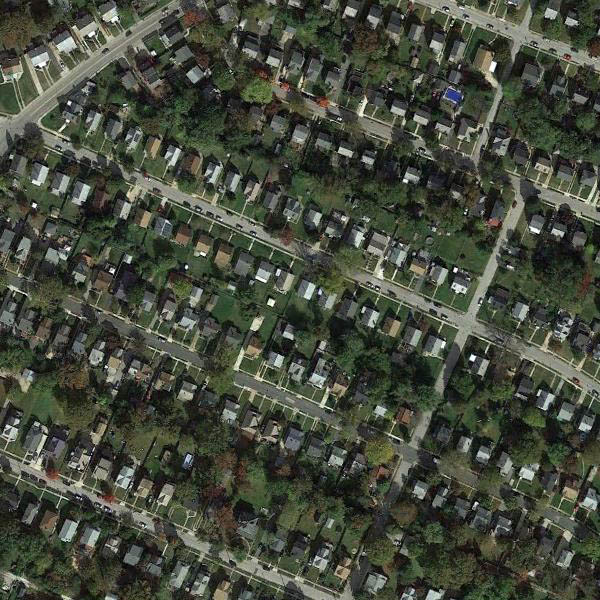
\includegraphics[width=0.65\linewidth]{AID/denseresidential_163.jpg}
                \caption{Área residencial distante}
            \end{minipage}
            \hspace{0.2cm}
            \begin{minipage}[b]{0.45\linewidth}
                \centering
                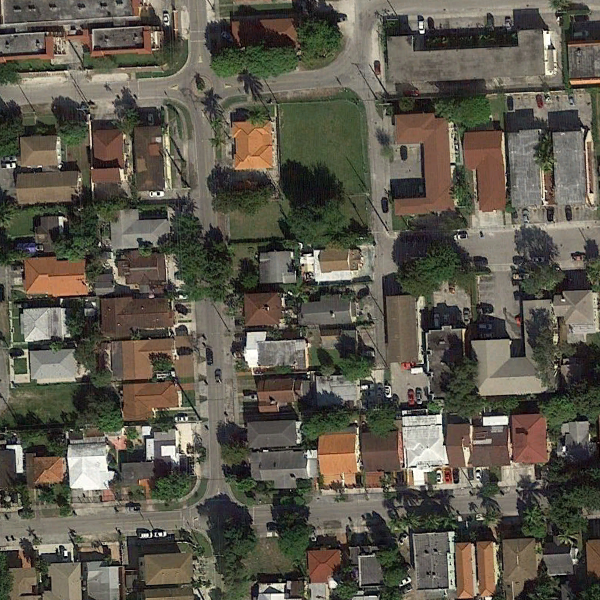
\includegraphics[width=0.65\linewidth]{AID/denseresidential_149.jpg}
                \caption{Área residencial próxima}
            \end{minipage}
        \end{figure}
        
    \end{frame}


    \begin{frame}{Quantidade de imagens e classes}
        \begin{itemize}
            \item 10.000 imagens com resolução \(600\times600\);

            \item Possui 30 classes;

            \item 220 a 420 imagens por classe, com média de 333;
            
            \item Airport, BareLand, BaseballField, Beach, Bridge, Center, Church, Commercial, DenseResidential, Desert, Farmland, Forest, Industrial, Meadow, MediumResidential, Mountain, Park, Parking, Playground, Pond, Port, RailwayStation, Resort, River, School, SparseResidential, Square, Stadium, StorageTanks, Viaduct
        \end{itemize}
    \end{frame}



    \begin{frame}{Exemplo de imagens}
        \centering
        % Primeira linha - 3 imagens
        \begin{minipage}[b]{0.3\linewidth}
            \centering
            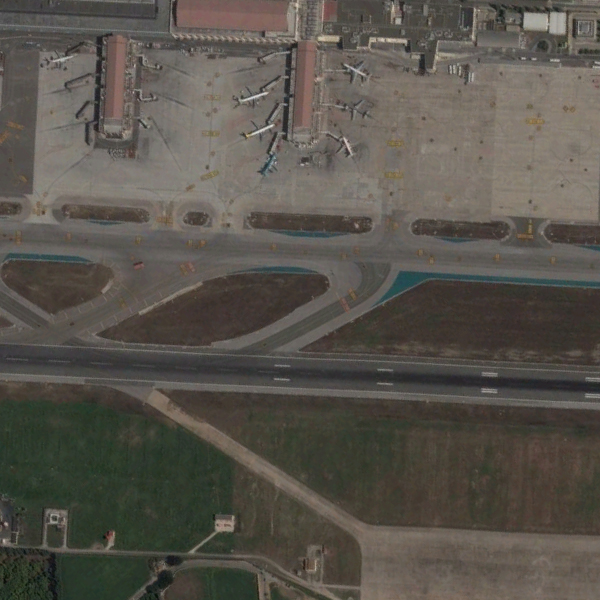
\includegraphics[width=\textwidth]{AID/airport_126.jpg}
            \scriptsize \textbf{\textit{Airport}}
        \end{minipage}
        \hspace{0.03\linewidth}
        \begin{minipage}[b]{0.3\linewidth}
            \centering
            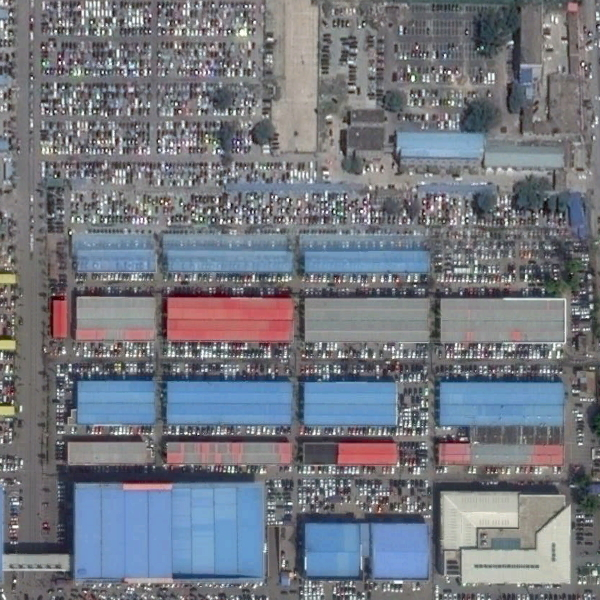
\includegraphics[width=\textwidth]{AID/industrial_12.jpg}
            \scriptsize \textbf{\textit{Industry}}
        \end{minipage}
        \hspace{0.03\linewidth}
        \begin{minipage}[b]{0.3\linewidth}
            \centering
            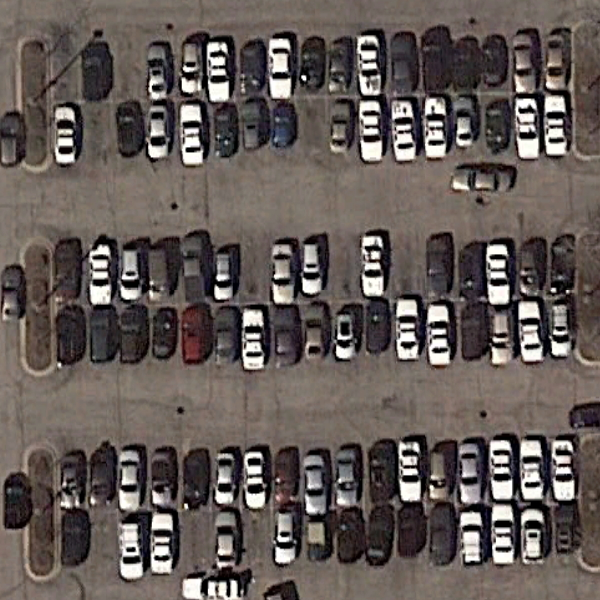
\includegraphics[width=\textwidth]{AID/parking_21.jpg}
            \scriptsize \textbf{\textit{Parking}}
        \end{minipage}
    \end{frame}
    
    \begin{frame}{Exemplo de imagens}
        \centering
        % Segunda linha - 3 imagens
        \begin{minipage}[b]{0.3\linewidth}
            \centering
            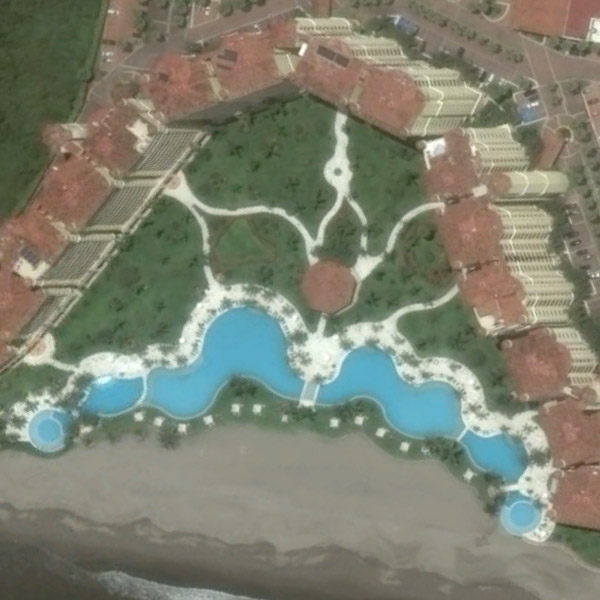
\includegraphics[width=\textwidth]{AID/resort_123.jpg}
            \scriptsize \textbf{\textit{Resort}}
        \end{minipage}
        \hspace{0.03\linewidth}
        \begin{minipage}[b]{0.3\linewidth}
            \centering
            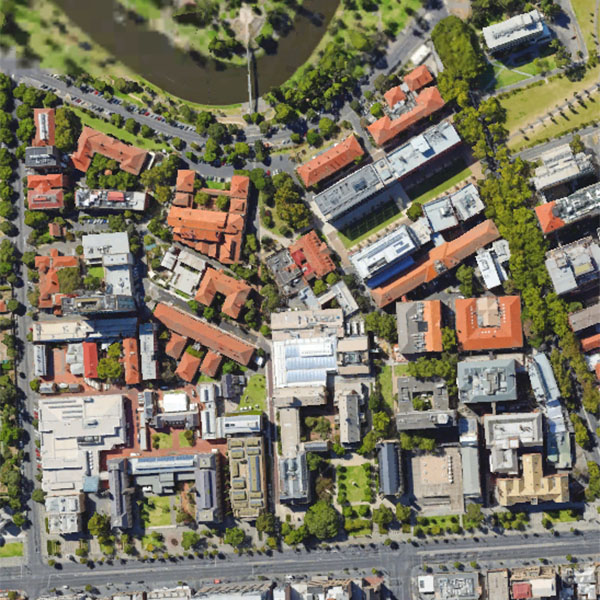
\includegraphics[width=\textwidth]{AID/school_66.jpg}
            \scriptsize \textbf{\textit{School}}
        \end{minipage}
        \hspace{0.03\linewidth}
        \begin{minipage}[b]{0.3\linewidth}
            \centering
            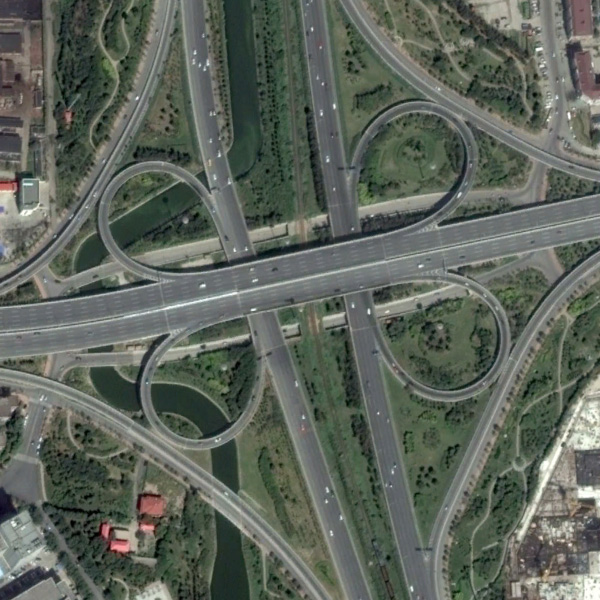
\includegraphics[width=\textwidth]{AID/viaduct_13.jpg}
            \scriptsize \textbf{\textit{Viaduct}}
        \end{minipage}
    \end{frame}






    \begin{frame}{AID}
        \begin{itemize}
            \item Alta variação intra-classe
        \end{itemize}
        \begin{figure}
            \begin{minipage}[b]{0.4\linewidth}
                \centering
                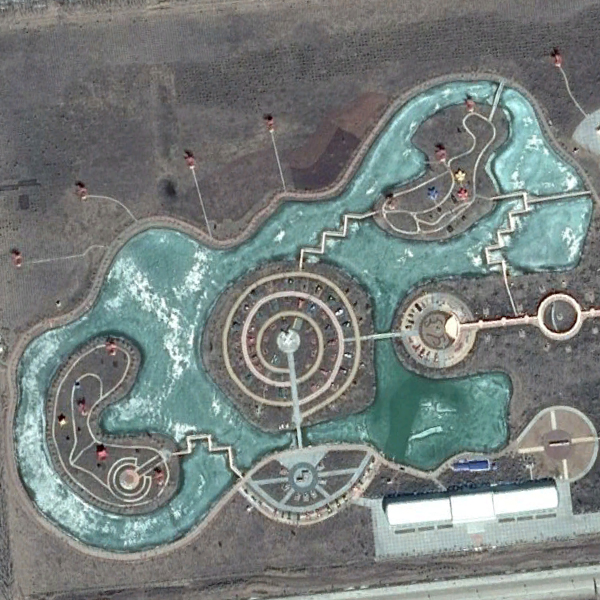
\includegraphics[width=0.9\linewidth]{AID/park_1.jpg}
            \end{minipage}
            \hspace{0.1cm}
            \begin{minipage}[b]{0.4\linewidth}
                \centering
                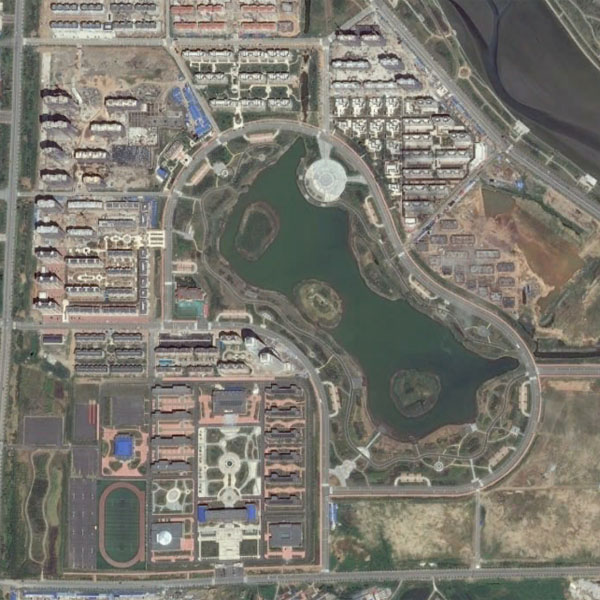
\includegraphics[width=0.9\linewidth]{AID/park_122.jpg}
            \end{minipage}
            \caption{Imagens da classe \textit{Park}}
        \end{figure}
    
    \end{frame}

    \begin{frame}{AID}
        \begin{itemize}
            \item Alta semelhança inter-classe
        \end{itemize}

        \begin{figure}
            \begin{minipage}[b]{0.4\linewidth}
                \centering
                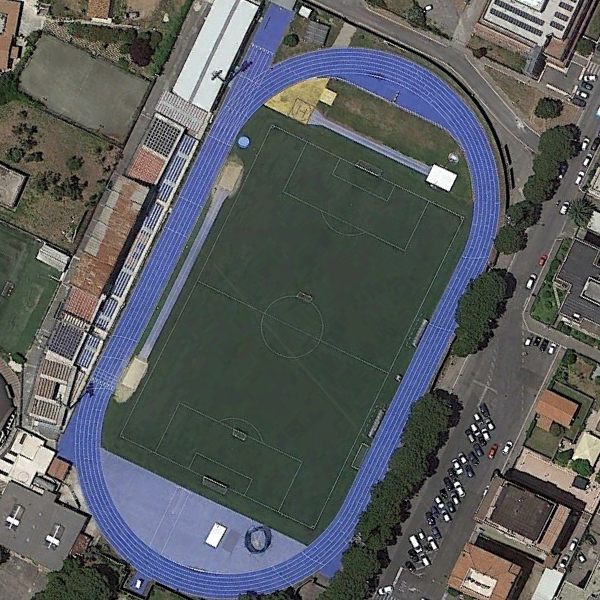
\includegraphics[width=0.9\linewidth]{AID/stadium_247.jpg}
                \caption{\textit{Stadium}}
            \end{minipage}
            \hspace{0.1cm}
            \begin{minipage}[b]{0.4\linewidth}
                \centering
                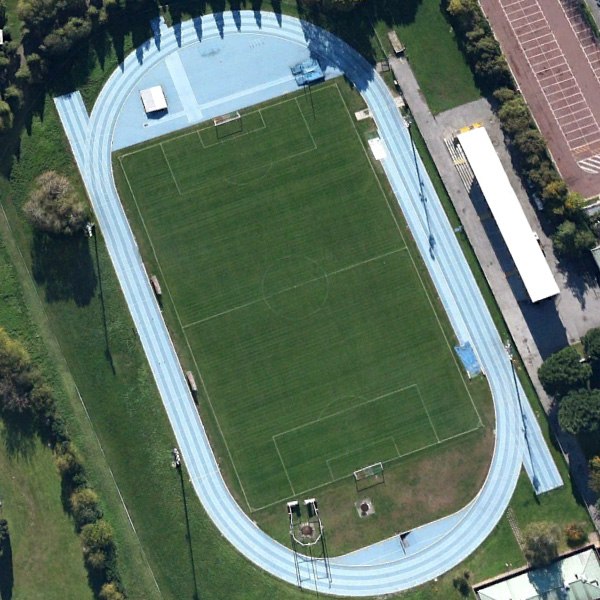
\includegraphics[width=0.9\linewidth]{AID/playground_184.jpg}
                \caption{\textit{Playground}}
            \end{minipage}
            
        \end{figure}
    \end{frame}
            